\section{Durchführung}

% wichtige zitierte wie \cite{nunes_systematic_2017} wurden trotzdem genommen.

\begin{figure}
    \centering
    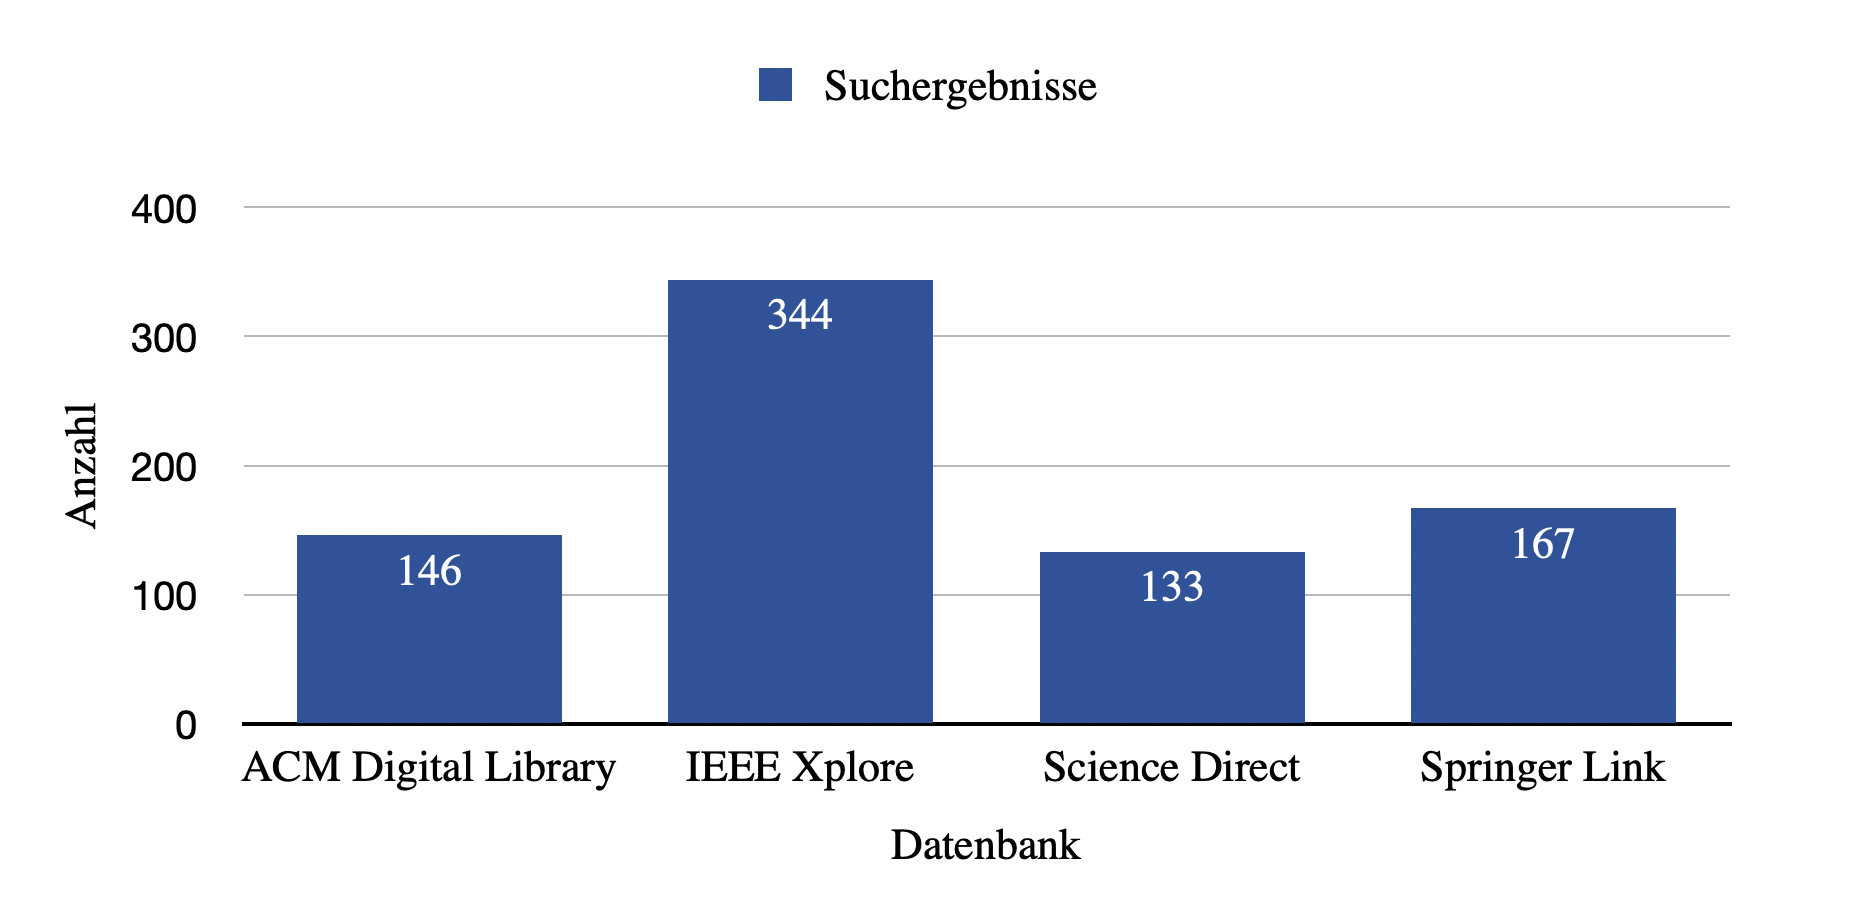
\includegraphics[width=0.75\linewidth]{contents/04_literature_review/res/database_results.png}
    \caption{Anzahl der Suchergebnisse pro Datenbank}
    \label{fig:04_literature_review_screening_process}
\end{figure}

\autoref{fig:04_literature_review_selection_process} bietet einen Überblick über das Auswahlverfahren der Arbeiten, auf denen die in dieser Arbeit entstandenen Ergebnisse aufbauen. Der Auswahlprozess ist in drei Iterationen erfolgt. Die Suche in den vier vorgestellten Datenbanken hat insgesamt 790 Arbeiten ergeben. Dabei gab es 141 Duplikate. Die initiale Menge der wissenschaftlichen Arbeiten nach der Suche enthielt folglich 649 Arbeiten. Da die Suche auf die genannten vier wissenschaftlichen Datenbanken beschränkt und bei der Suche bereits die Filter passenden Filter genutzt wurden, erfüllen diese Veröffentlichungen bereits alle die Kriterien des \textit{Peer Review} und \textit{Pre-Prints} ([I1], [E3]).

\begin{figure}
    \centering
    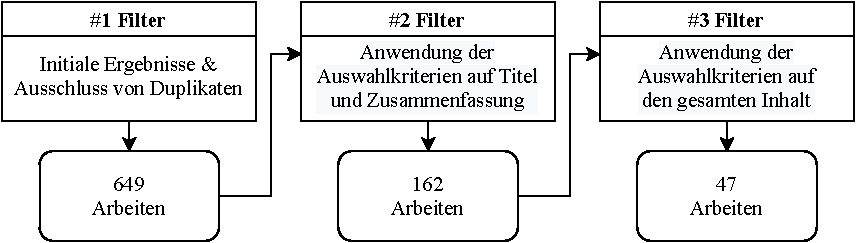
\includegraphics[width=\textwidth]{contents/04_literature_review/res/selection_process.pdf}
    \caption{Auswahlverfahren der Literaturrecherche}
    \label{fig:04_literature_review_selection_process}
\end{figure}